\documentclass[onecolumn,10pt]{IEEEtran}

\usepackage{graphicx}
\usepackage{siunitx}
\newcommand{\myroot}{../}
\newcommand{\Later}{\textbf{Later.}}

\title{Autonomous Drone Racing}
\author{A.~Credle and D.~Evangelista\thanks{Authors are with the United States Naval Academy, Department of Weapons, Robotics, and Control Engineering}}
\date{today}

\begin{document}
\maketitle

\begin{abstract}
Abstract here. \Later
\end{abstract}

\section{Background and motivation}
\Later

\section{Problem statement}
%I have a problem. No it seems to work now. 
Given a small quadrotor drone with an inertial measurement unit (IMU) and a single camera, this research intends to begin the process of developing autonomous drone flight through a drone racing course. Given both a preloaded three dimensional path,  we will find and test the feasibility of a guidance system that collaborates computer vision with the preloaded path. This system will be tested by placing a small quadrotor in multiple scenarios in relation to a race gate(s), with varying angles of approach and gate sizes, and directing the guidance system to fly the drone through the race gate(s). Success of this system is having the drone autonomously fly through multiple race gates(?) without contact in every scenario given at the drones maximum horizontal speed. The final output of this project will a guidance system that could be implemented on any racing drone with a camera and IMU and fly through multiple race gates. 
\begin{figure}[h]
\begin{center}
\includegraphics[width=4in]{\myroot/figures/racegate-intro.png}
\end{center}
\caption{A quadcopter drone flying through a racing gate.}
\label{fig-problem-statement-1}
\end{figure}

\section{Literature review}
\Later\ This paper is the one of the first developments of a drone autonomous flight program, so the background research encompasses papers that focus on multiple aspects of autonomous flight. The main categories that these papers fall into include navigation, flight controls, and visual recognition. This research focuses on the visual recognition of the gate, but these other two categories are necessary for the background research because they affect the performance of visual recognition and are necessary for basic demonstration. 

In order to understand the movement patterns of the drone, \cite{svacha2017improving} provides a set of equations that could be used to accurately model the induced drag and thrust forces. These equations were derived from proofs using properties of physics, and then the coefficients were identified through flight experimentation. This allows provides suitable estimations for the forces acting on the drone, which allows for control of the drone through the gate. This is connected to \cite{loianno2017estimation}, which created a state equation set that could accurately model the movement of a small drone with aggressive flight. By determining these equations through modeling and live testing, these state equations can be coupled with the flight force equations from \cite{svacha2017improving} to form an accurate estimate of the drones location. Coupling these with a flight controller will allow the drone to have a basic understanding of its location as compared to the general space. This research is centered around coupling visual servoing and preprogrammed flight paths, and in order to understand the drones relation to the preprogrammed flight path, \cite{svacha2017improving} and \cite{loianno2017estimation} provide an accurate location. 

While \cite{svacha2017improving} and \cite{loianno2017estimation} provide what is believed to be an accurate location of the drone in-flight, it’s location in relation to the preprogrammed flight path isnt always certain. \cite{florence2018nanomap} provides the groundwork for a concept known as Nano Mapping, which refers to modeling a 3D data structure depicting obstacles around the drone. This technique is different from a traditional mapping approach because tradtional mapping is based of a common world frame. \cite{florence2018nanomap} is based solely on the frame of the drone, allowing for a calculatable uncertainty to enter trajectory planning. This concept is also crucial to the development of this research because the coupled flight path planning approach requires both the common world frame and the drone world frame.

Different methods for seeing the world around the drone exist, including range finding technology (used for altitude measurements), single camera, and multi camera approaches. \cite{loianno2017estimation} is based on a single camera approach, while \cite{zhilenkov2018use} found that a three camera setup was optimal for uncertain terrains. \cite{zhilenkov2018use} is based on autonimous navigation of drones in a wooded area, where to location of the trees is unknown before flight, and path recognition is taught to the drone using AI. While the racecourse for this research is assumed to be known, a single camera apporach will be utilized for hardware simplicity; the AI approach of path recognition, however, may be utilized in this research’s gate recognition technology. If a neural network could be constructed to follow a path through a forest, a similar neural network could be formed to fly through an ariel path.

One of the main challenge that arises with flying through the gate is recognizing multiple gates. In small drone racing courses, it is likely that the drone will be able to see multiple gates within its field of view. \cite{jung2018perception} worked through this problem and found resonable neural network perameters to mitigate this issue. By assuming the next gate in the racecourse would be the largest gate in the drone camera view (using a single camera approach), \cite{jung2018perception} removed the nueral network layer of all image analysis and left only the recognition of the largest circle gate. By removing this process in the image analysis, \cite{jung2018perception} found a significant increase in processing power while only reducting the accuracy of gate recognition by less than \SI{10}{\percent} (\SIrange{464}{34}{\milli\second} reaction time, \SIrange{82.4}{75.5}{\percent}).

The other main challenge that arises after roecognizing the proper gate to fly through is implementing a visual servoing program to direct the drone through the gate. \cite{jung2018direct} created a process of gate recognition that located the center of the gate in relation to the location of the center of the cameras view and redirecting the drone towards the center of the gate. This background research is the closest process to the research in this paper, as it specificies a visual recognition procesc that is simplified into the computational level of an inflight processor.

While many of these papers are useful in the development of an autonimous drone, it should be noted that there lacks a consistancy among drone researchers in the underlying assumptions. As described earlier, some researchers utilize a single camera operating system, while others use multi-camera systems, and even some include range finding technology. Many of the subjects of these papers devled into different subsections of drone autonomy, so it is reasonable that their methods varied, but many of these research projects should have been underwent with a more uniform drone system in place for practicality. For research such as \cite{svacha2017improving}, \cite{loianno2017estimation}, and \cite{florence2018nanomap}, their research was more for drone flight in general, so this critique doesn’t apply as much as it does for projects such as \cite{zhilenkov2018use}, \cite{jung2018perception}, and \cite{jung2018direct}, which had varying sensor and visual capabilities. As the latter 3 projects had more to do with direct visual recognition, it would have been more advantageous for the autonimous drone community had the projects been embarked on in a similar manner.

These projects center around the research in this proposal in two ways: by giving basic flight control and navigational equations to use in baseline location estimations and flight controllers, and by providing simplistic approaches to visual recognition to model my approach. While my approach uses both a whole world frame and a drone view frame to form a novel approach to gate recognition, many of the approaches depicted in \cite{zhilenkov2018use}, \cite{jung2018perception}, and \cite{jung2018direct} can be used to model a realistic approach to melding the two frames. This project will take these simplistic approaches and form a simple and novel approach to visual gate recognition.






\section{Demonstration plan}
\Later\ In this project, it is important to ensure that factors not related to gate recognition do not hamper the performance of the drone. With small quadcopters performing advanced maneuvering, it can be difficult to predict and measure its exact movements, which could negatively affect this projects ability to test gate recognition capabilities. While not optimal for a project focused on practicality, initial testing will be conducted in drone flight simulators. This will ensure that gate recognition processes can be focused on before moving to actual flight-testing.

In order to demonstrate the effectiveness of the gate recognition process, a mix of simulations and experiments will required. First, simulations will be run to give the AI enough examples to test its understanding of what a gate looks like, so the same simulation can be used to show the AIs theoretical accuracy. Secondly, a simulated course will be run in order to demonstrate ideal drone capabilities with mixed flight and gate recognition programming. Last, a physical experiment with a small, single camera quadcopter with an internal IMU will be sent through a variety of racecourse configurations to ensure its practicality.

%\subsection{Mathematical analysis}

\subsection{Simulation or computational studies}
As stated previously, simulation will be relied on heavily before moving into experimental work. This is to ensure that any unknown external factors do not interfere with the gate recognition process. This is critical because if there are adjustments required upon final testing, testing in simulation will allow for quick specific adjustments. In addition, this allows for testing to be run at a speed exponentially faster than a physical test.

Simulation testing for the first two sections of the demonstration is necessary because of its control, replicability, and generality. In the drone flight simulators, a myriad of flight controls can be controlled with the click of a button. Every movement of the drone will be calculated and ideal. This is optimal for initial demonstrations for two reasons. First, it allows for exact movements, so the drones flight can be programmed simply. For example, if gates are introduced into the simulation directly in front of the drone, the simulation can be programmed to fly the drone straight through the gates without having to worry about altitude loss, wind factors,drag, etc. On a very basic level, the drone can be programmed to fly a perfectly straight line. While this is not realistic to real world environments, it is useful for initial gate recognition. Secondly, this test can be replicated thousands of times an hour. If thousands of test runs are collected, we can product an accuracy rating for the gate recognition processes, and failed test runs can be analyzed for process alterations.

While recognizing a gate head on in a simulated environment may not be incredibly difficult, a new challenge will be added to test the recognition software. The bigger challenge is having the drone recognize gates from non-ideal angles. In cases where a drone approaches a gate at an increased angle, it is assumed that the recognition processes will struggle. Identifying a pure circle is easy, however recognizing a small ellipse and accurately predicting an approach angle that allows the drone to fly through the gate without hitting either gate edge is more challenging. By running simulations where thousands of angles can be tested, this allows for a complete understanding of the image processing capabilities. This, again, is not the most realistic test, but it allows for complete control of the drones flight, and can be replicated thousands of times over. By creating a general understanding of the drones response to different situations, troubled situations can be mitigated and a more accurate physical experiment can be implemented.

\subsection{Experimental work}
The second phase of demonstration for this project includes proof-of-concept experiments of a drone flying through single and multi-gate racecourses. First, a single gate course will be created in order to test basic gate recognition processes alongside flight controllers. The drone will be set to take off from a flat surface, recognize a gate placed in front of it, fly through the gate, and then land on a flat surface. The test will then be modified by moving the gate from directly in front of the drone to different locations so the drone can be shown recognizing and flying through different approach angles. Next, a multi gate course will be created (2--5 gates) in which the drone will fly through the gates in sequential order. Sequential order is important as it shows the recognition programs capability of distinguishing which gate is closer, in turn recognizing the correct order of gates. While initial multi gate testing will be conducted with the gates in a straight line, the gates will eventually be configured in curved and staggered patters (see Figures~\ref{fig-gate-style-1} and \ref{fig-gate-style-2} below). These tests are the closes to drone racing that this project will go, as demonstrating multi-gate recognition is subsequent for basic drone racing. In the future, this project could be utilized for a high speed-racing drone, which would need better flight recognition capabilities (seeing gates at long distances or flying towards gates outside of the cameras line of sight), but for this project, simple gate testing will be sufficient.
\begin{figure}
\caption{Depiction of multi-gate racecourse style 1}
\label{fig-gate-style-1}
\end{figure}

\begin{figure}
\caption{Depiction of multi-gate racecourse style 2}
\label{fig-gate-style-2}
\end{figure}

For the physical experiments, standard drone racing specifications will be maintained. Lockheed Martin currently has a drone racing competition, known as the AlphaPilot Challenge, which requires specific drone specifications (power supplies, drone size, motor power, etc.). As these specifications are published, they will be maintainedwithin this project, and it is assumed that these specifications will meet the requirements for powering, computing, and sensing within this project.

\subsection{Property measurement}
As this is the first phase within the many steps required for functional autonomous drone racing, it is assumed that the results from this project will be close to the results of current research. As seen in \cite{jung2018perception}, the accuracy of AI integrated gate recognition using large off-board computers was found to be between \SIrange{75}{85}{\percent} gate recognition accuracy. This data was taken at full flight speeds (\SIrange{4}{5}{\meter\per\second}), while this project is not focused on speed, so it is assumed we will have similar accuracies. In order to compare our results to those of other researchers in the gate recognition field, a gate recognition accuracy measurement is necessary. This is comprised of the number of gate correctly recognized in the proper order divided by the number of gates the drone is presented.

\subsection{Technical risks and mitigation}
Due to the innate troubles with high-speed drone flight, there is always the risk of crashing a drone. In our experiments, we plan to minimize this risk by keeping speeds significantly lower than racing speed (\SIrange{0.5}{5}{\meter\per\second}). In addition, there is a collection of drones from past swarm projects available, so excess batteries and drones are available in the event that batteries die or drones crash and break. While there may be technical issues with building drones specific to the AlphaPilot Challenge, the instructions provided with the drone building class at USNA are easily accessible, so issues with drone building and drone flight should be minimal. The only other issue that may arise is low battery life, which will be mitigated by the batteries available at USNA, or will be budgeted for (this will be known by the budget section due date).

%\subsection{Time risks and mitigation}
%\subsection{Justification of high risk activities}
%\subsection{Budget}
%\begin{table}[hb]
%\caption{Budget}
%\label{table-budget}
%\end{table}

\section{Conclusion}
\Later

%\section*{Acknowledgements}
%\addcontentsline{toc}{section}{Acknowledgements}

\bibliographystyle{IEEEtran}
\bibliography{IEEEabrv,\myroot/references/credle}
%
%\appendix
%\section{Gantt Chart}
%\Later\ Insert the Gantt chart here. Be sure the font is legible. Crop it tight, use landscape orientation and make it as large as possible.
%

\begin{IEEEbiography}[{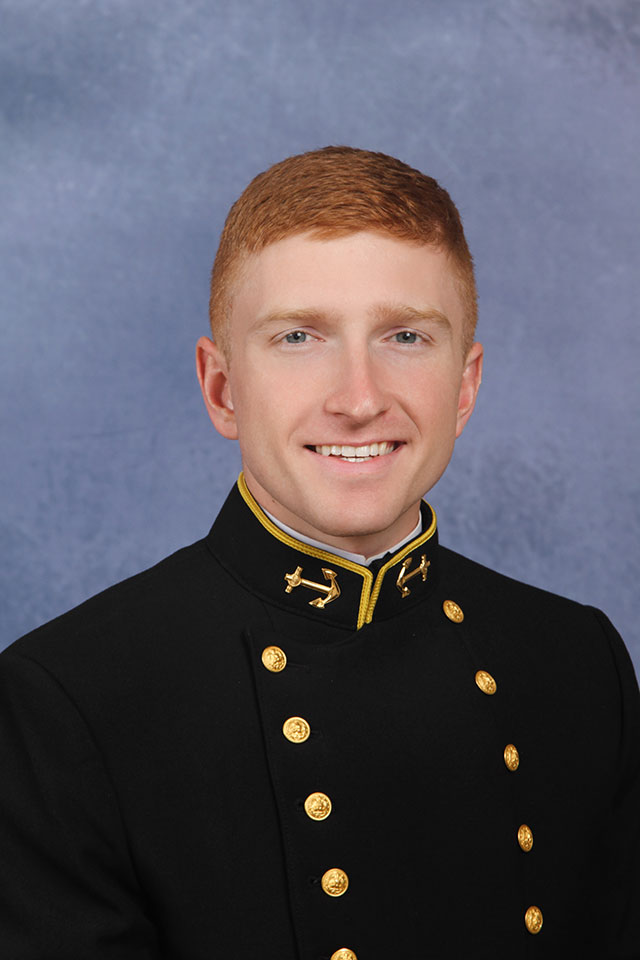
\includegraphics[width=1in,height=1.25in,clip,keepaspectratio]{\myroot/figures/M201260.jpg}}]{Austin Credle} is a midshipman at the United States Naval Academy majoring in Robotics and Control Engineering. Upon graduation, he hopes to service select as into either the pirate/privateer or blimp communities. 
\end{IEEEbiography}

\begin{IEEEbiography}[{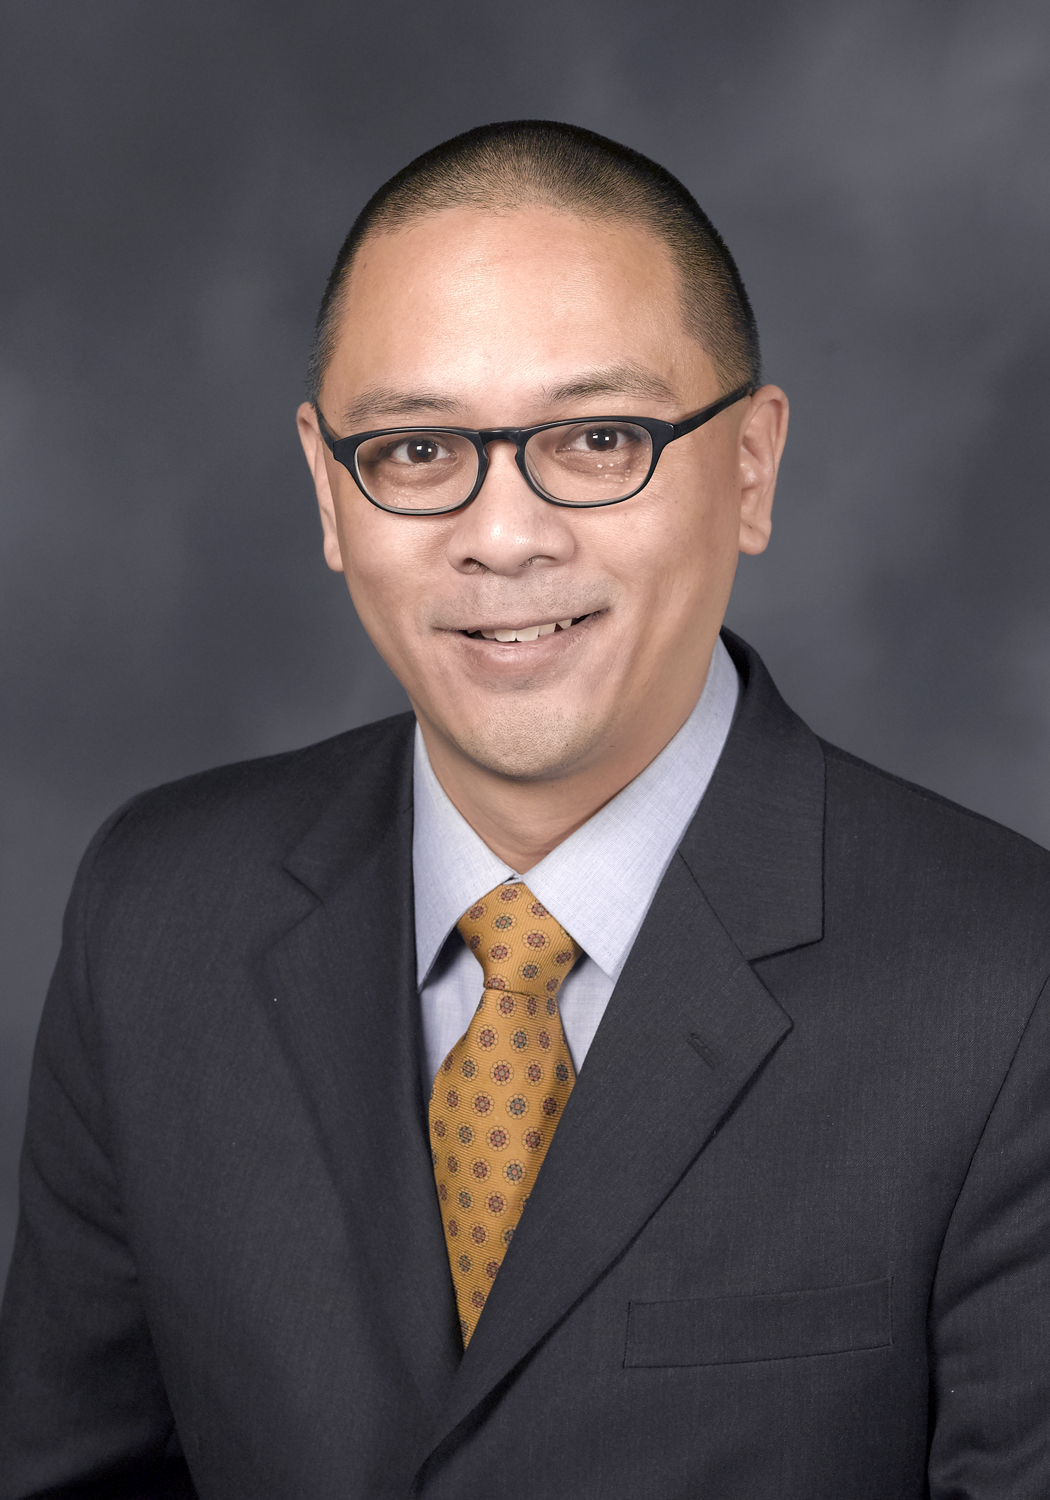
\includegraphics[width=1in,height=1.25in,clip,keepaspectratio]{\myroot/figures/evangelista_d_prof.jpg}}]{Dennis Evangelista} raises guide dog puppies. 
\end{IEEEbiography}

\end{document}